% !TeX root = ../main.tex
% Add the above to each chapter to make compiling the PDF easier in some editors.

\chapter{Related Works}\label{chapter:related_works}

\section{Fault feature extraction for DL-based Predictive Maintenance}
Nonstationary signal analysis, which refers to investigating signals with changing statistical properties over time, is one of the main topics in the field of machinery fault diagnosis. Signals can contain multiple frequencies and change their amplitude while traveling in time. Traditional signal analysis techniques make stationary assumptions. When applying those just on non-stationary signals statistical averages in time or frequency are be extracted \cite{FENG2013}. The demand for analysis methods, which allows ascertain features of such non-stationary signals is increasing. Especially for collecting machine health related information, these methods seem to be promising. Traditionally, Fourier transforms are an important tool in signal analysis. The Fourier transform relates the one-dimensional time- and frequency domains as following:

\begin{equation}
    \begin{aligned}
        & \mbox{time-domain (signal):} \\
        & x(t) = \int_{f} X(f) e^{j 2 \pi t f} df \\
        & \mbox{frequency-domain (spectrum):} \\
        & X(f) = \int_{t} x(t) e^{- j 2 \pi f t} dt, \\
    \end{aligned}
\end{equation}

Since both domains are not combined but just related, the time specific information are lost in the frequency domain and the other way round. The relation between the time- and frequency domain created by the Fourier transformation is visualized in fig. \ref{fig:fourier} 
\begin{figure}[H]
  \centering
  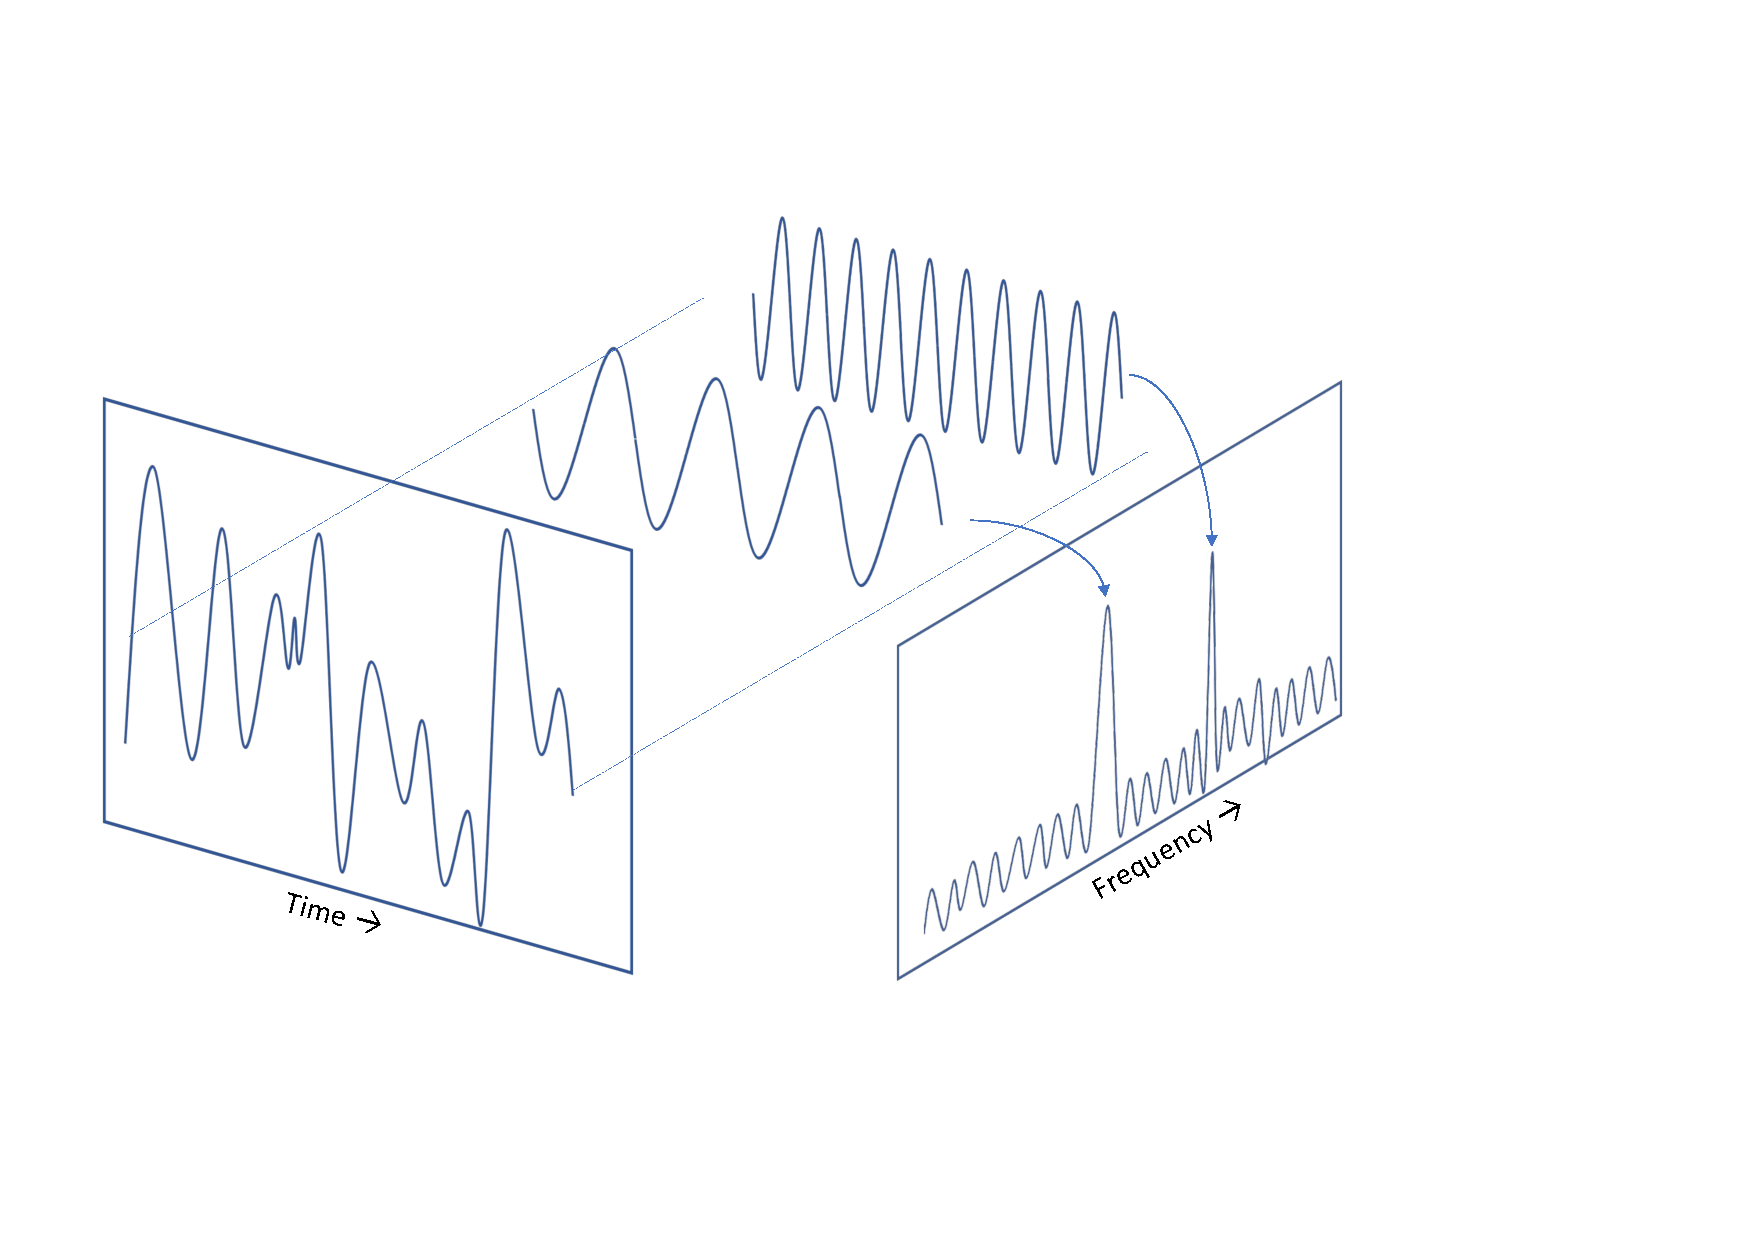
\includegraphics[width=.75\textwidth]{preprocessing_transform/fourier.pdf}
  \caption{Relation between time- and frequency domain through Fourier transformation}
  \label{fig:fourier}
\end{figure}

Time–frequency representations (TFR) solve this problem by transforming the one-dimensional signal in two-dimensional time-frequency plane, where each value corresponds to the dominance of a specific frequency at a certain point in time. Mathematically the two-dimensional data is represented by the joint function $T_{x}(f,t)$, where $x$ is the data of interest and the arguments of the function is the time  $t$ and frequency  $f$. One separates different methods of this type by the relation dependency of $T_{x}(f,t)$ on the input signal $x(t)$. There exist linear, quadratic or non-linear relationships. The focus of this chapter is to describe linear and quadratic TFRs in more detail \cite{Hlawatsch1992}. 

\subsection{Linear time–frequency representations}
When the signal of interest can be decomposed in several linearly related components then the TFR of this signal can also be expressed as a linear combination of TFRs corresponding to each signal component:
\begin{equation}
    \begin{aligned}
        x(t) = c_{1} x_{1}(t) + c_{2} x_{2}(t) \rightarrow T_{x}(f,t) = c_{1} T_{x_{1}}(f,t) + c_{2} T_{x_{2}}(f,t)
    \end{aligned}
\end{equation}


All TFRs which fullfill this idea of linearity and superposition are called linear TFRs. The two most popular linear TFRs are the short-time Fourier and Wavelet transform \cite{Hlawatsch1992}. 
\subsubsection{Short-time Fourier transform}

Short-time Fourier transform (STFT) is a method which adds a time variable to the traditional Fourier spectrum. This allows to investigate variations in the signal's spectrum over time. STFT assumes the spectrum to be constant during a short time window. For each such window a Fourier spectrum is obtained and the time related changes are measured between such consecutive snapshots in the data. Window functions are defined which separate the signal. For each window a Fourier transform is applied. The process is mathematically expressed in the following:  
\begin{equation}
    STFT_{x}(t,f) = \int_{- \inf}^{+ \inf}x(\tau) w(\tau -t) exp(-j2\pi f \tau),
\end{equation}
where  $w(\tau -t)$ is the window function centered around t which is multiplied with the signal $x(t)$. Shifting the window over the signal and applying the Fourier transform $exp(-j2\pi f \tau)$ generates a local frequency spectrum of the signal for different points in time t \cite{FENG2013}. The time-frequency resolution is defined by the windowing function and the window length. STFT suffers from a trade-off between high resolution in time or in frequency. The optimum window length will depend on main interest behind the signal analysis. For accurate time domain information the window size needs to be reduced and for frequency domain information increased. STFT  decomposes the signal in existing sinusoidals and determines it's frequency and phase for a local part of the signal \cite{Hlawatsch1992}. 

\subsubsection{Wavelet transform}
The Wavelet transform decomposes the signals in several wavelets which contain information about the health condition of the machine. A wavelet is a wave-like oscilation which is described by it's function, location and scale. The location defines where the wavelet overlaps with the signal and the scale defines how much squished (small scale) or stretched (big scale) the wavelet is. The wavelet is shifted along the signal by changing it's location. At each of it's position the wavelet is convolved with the signal \cite{Shawhin2020}. The convolution of the wavelet and the signal is mathematically expressed as following:
\begin{equation}
    WT_{x}(t,a) = \frac{1}{\sqrt{a}} \int_{- \inf}^{+ \inf} x(\tau) \psi(\frac{\tau -t}{a}) d \tau,
\end{equation}
 where $x(t)$ is the signal which is convolved with the wavelet $\psi(\frac{\tau -t}{a})$. In this case $a$ is the scaling factor, $t$ is the time shift and $\frac{1}{\sqrt{a}}$ is a normalization factor to maintain the energy conservation \cite{FENG2013}. Different wavelet bases $\psi(t)$ can be convolved with the signal. This helps to analyze the signal for different pattern, which have similar properties as the wavelet \cite{Shawhin2020}. Possible wavelet bases are be the Gaussian, Morlet, Shannon, Meyer, Laplace, Hermit, or the Mexican Hat wavelets in both simple and complex functions \cite{Verstraete2017}. This allows a more extensive, flexible and detailed analysis. In fig. \ref{fig:ricker_wavelet} Ricker wavelets with different scales and locations are visualized. Wavelet transforms can extract local spectral and temporal information in parallel \cite{Shawhin2020}.


\begin{figure}[H]
  \centering
  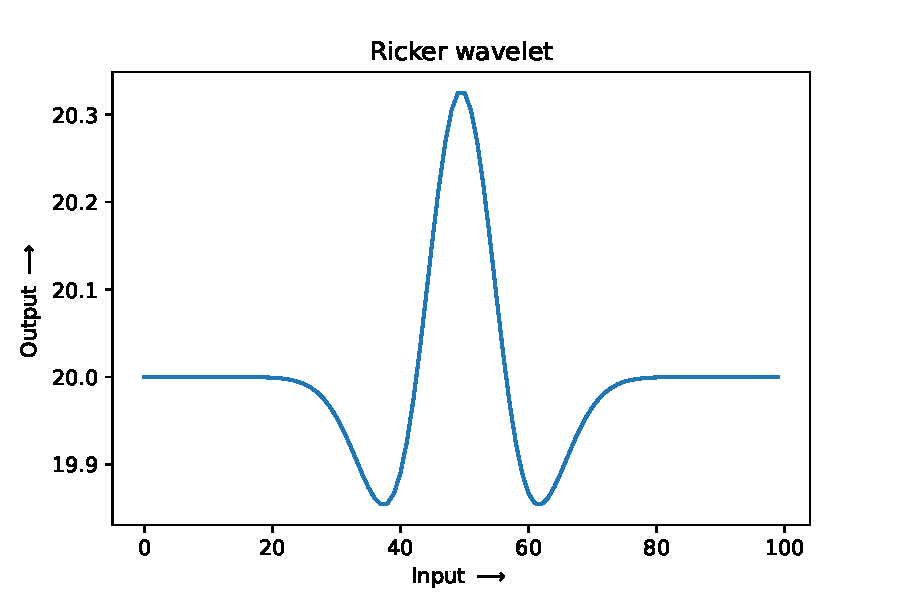
\includegraphics[width=.47\textwidth]{preprocessing_transform/wavelet_small_scale.pdf}
  \hspace{.1cm}
  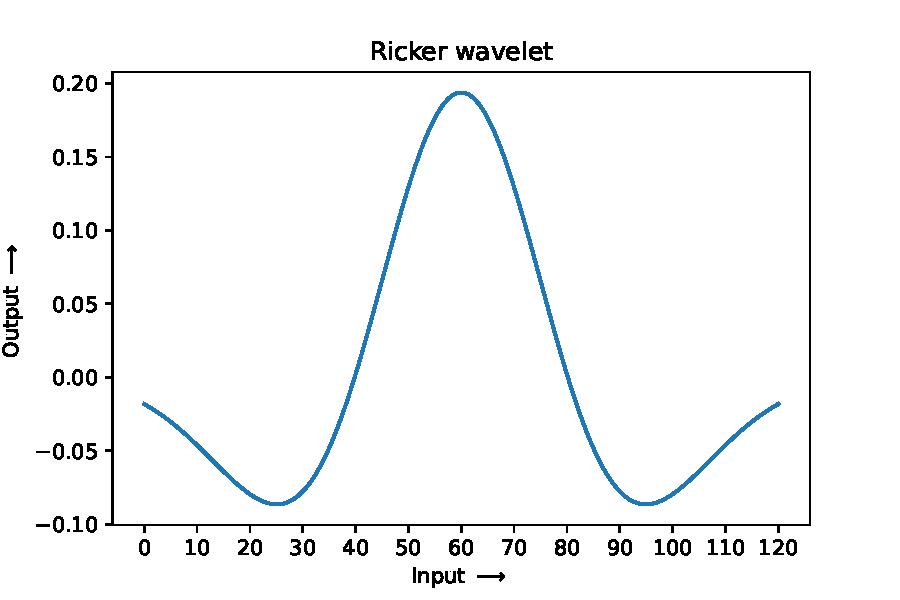
\includegraphics[width=.47\textwidth]{preprocessing_transform/wavelet_big_scale.pdf}
  
  \vspace{.1cm}
  
  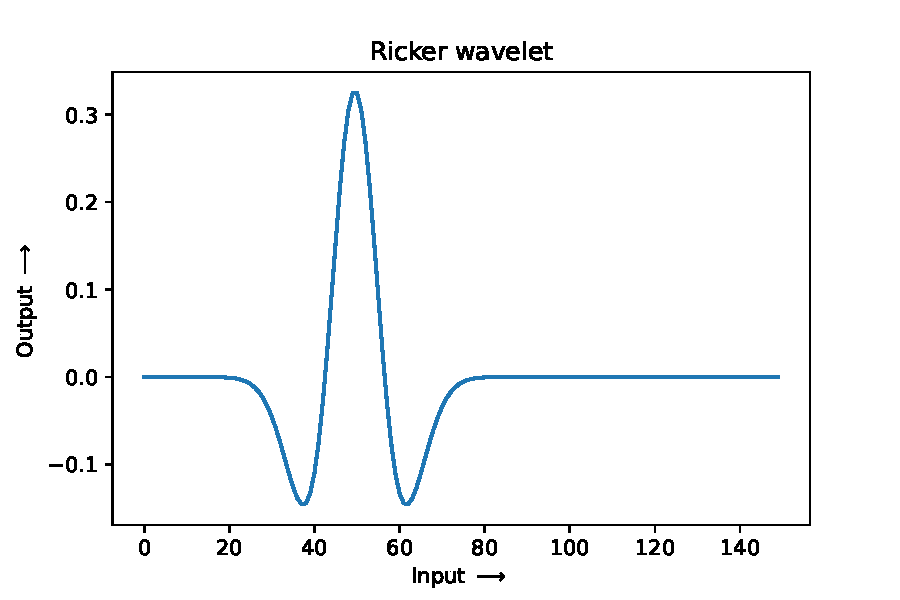
\includegraphics[width=.47\textwidth]{preprocessing_transform/wavelet_left_scale.pdf}
  \hspace{.1cm}
  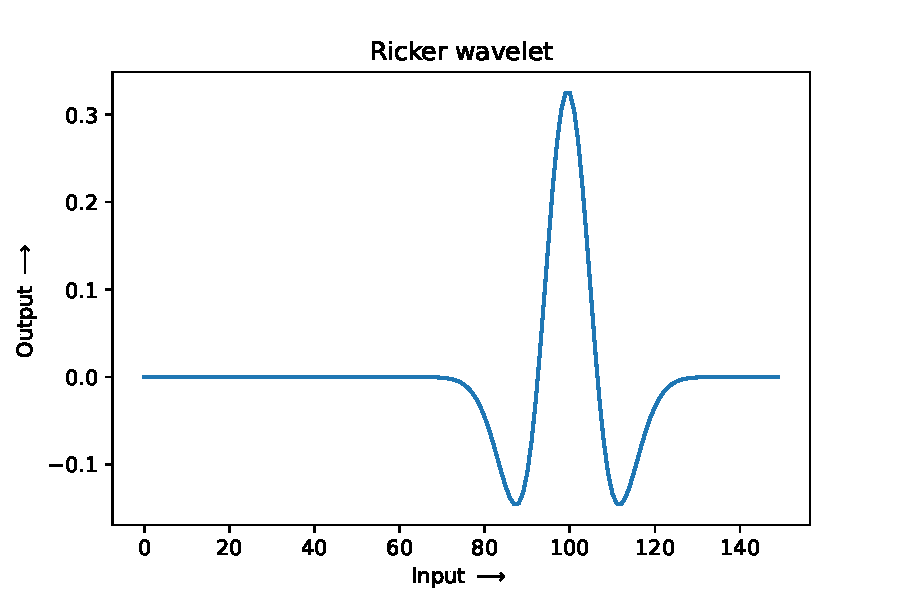
\includegraphics[width=.47\textwidth]{preprocessing_transform/wavelet_right_scale.pdf}

  \caption{Ricker wavelet with different scale (top) and shifting (bottom) factors}
  \label{fig:ricker_wavelet}
\end{figure}

\subsection{Spectrograms and Scalograms}

 Spectrograms are a graphic representation of the STFT and scalograms of the wavelet transform. Spectrograms and scalograms visualize the the squared magnitudes of the previously presented STFT and Wavelet transform. This squared magnitude are loosly interpreted as signal energy \cite{Hlawatsch1992}. The mathematical expressions are presented in the following: 

\begin{equation}
    \begin{aligned}
        &SPEC_{x}(t,f) = \abs{STFT_{x}(t,f)}^{2} \\
        &SCAL_{x}(t,f) = \abs{WT{x}(t,f)}^{2}, 
    \end{aligned}
\end{equation}

where $STFT_{x}(t,f)$ is the Short-time Fourier transform, $WT_{x}(t,f)$ the wavelet transform, $SPEC_{x}(t,f)$ the spectrogram and $SCAL_{x}(t,f)$ the scalogram \cite{Hlawatsch1992}. This way of representing the system energy in the 2d time and frequency space may reveal useful information from the complex and high-dimensional data without the need for additional feature extraction. As described before spectrograms have a fixed frequency resolution that is defined by the windows size. Scalograms on the other hand have a frequency- dependent frequency resolution \cite{Verstraete2017}.

\subsection{Adaptive non-parametric time–frequency analysis}
Adaptive non-parametric approaches include empirical mode decomposition (EMD) \cite{FENG2013}. Unlike other multiresolution analysis (MRA) techniques such as wavelet analysis EMD recursively extracts Intrinsic Mode Functions (IMF) from a non-stationary time series. According to Faltermeier et al. \cite{Faltermeier2010} IMFs have the following properties: 

\begin{itemize}
    \item [1] An IMF has just one extremum between to zero crossings. Local minima and maxima do need to alternate such that the number of local minima and maxima does differ at most by one. 
    \item[2] An IMF need to have zero mean, but still the IMF can have changing frequencies and amplitude modulation. 
\end{itemize}

The EMD algorithm decomposes the signal as following:

\begin{equation}
    x(t) = \sum_{n} x_{n}(t) + r(t),
\end{equation}
where $x(t)$ is the signal, $x_{n}(t)$ the n-th IMF and $r(t)$ the residuum \cite{Faltermeier2010}. Faltermeier et al. \cite{Faltermeier2010} describte the recursive extraction of IMFs from the signal as following: 
\begin{itemize}
    \item [Step 0:] Initialize: $n := 1$, $r_{0}(t) = x(t)$
    \item [Step 1:] Extract the n-th IMF as follows:
    \begin{itemize}
         \item [a)] Set $h_{0}(t) := r_{n−1}(t)$ and $k := 1$
         \item [b)] Find all local maxima and minima of $h_{k−1}(t)$
         \item [c)] Construct envelopes for all the identified maxima $U_{k−1}(t)$and minima $L_{k−1}(t)$ for $h_{k−1}(t)$ using cubic interpolation
         \item [d)] Determine the mean $m_{k−1}(t) = 12 (U_{k−1}(t) - L_{k−1}(t))$ of both envelopes of $h_{k−1}(t)$.
         \item [c)] Form the k − th component $h_{k}(t) := h_{k−1}(t) - m_{k−1}(t)$
         \begin{itemize}
            \item [i)] if $h_{k}(t)$ is not in accord with all IMF criteria, increase $k \rightarrow k + 1$ and repeat starting at step b
            \item [ii)] if $h_{k}(t)$ satisfies the IMF criteria then set $x_{n}(t) := h_{k}(t)$ and $r_{n}(t) := r_{n-1}(t) − x_{n}(t)$
         \end{itemize}
    \end{itemize}
    \item [Step 2:] Check another IMF needs to be extracted
        \begin{itemize}
            \item [i)] if $r_{n}(t)$ is the residue, the original data is decomposed in the n IMFs  $x_{n}(t)$ and the residue $r_{n}(t)$
            \item [ii)] if $r_{n}(t)$ is not the residue, go to Step 1.
         \end{itemize}
\end{itemize}


The number of IMFs extracted roughly equals $log_{2}(N)$ where $N$ is the number of extrema in the signal. The EMD decomposes the non-stationary signal in its locally and non-overlapping component IMFs. This process does not need any predefined wave-forms like the wavelet transformations. The selection of the IMFs is an automatic and adaptive time-variant filtering \cite{Faltermeier2010}. Compared to the Fourier and Wavelet transform, the decomposition of the signal in several IMFS does not divide the signal into fixed frequency components, which gives this method a higher time-frequency resolution \cite{Verstraete2017}. The popular Hilbert-Huang Transform (HHT) combines the EMD with the Hilbert spectral analysis, where the Hilbert transform is applied to each of the detected IMFs. A corresponding analytical signal can be constructed. Also the Hilbert amplitude and energy spectrum can be derived. For more Hilbert-specific details Feng et al. \cite{FENG2013} can be studied.

\section{Domain adaptation approaches for Predictive Maintenance (PM)}
In recent years, intelligent data-driven machine condition monitoring systems have replaced traditional approaches to a great extent. When using such monitoring systems for long time horizons operational conditions and therefore fault characteristics might change. This leads to unsatisfactory diagnosis performance \cite{AZAMFAR2020103932}. Furthermore, there are scenarios where not all fault classes are known during training. Due to the correlation and dependency between different parts of the system, faults can have numerous causes and can influence the systems in different ways. Therefore it is unlikely that the data used for training the model includes all system states and fault scenarios. PM systems which can handle unseen fault classes and robustly handles variations in fault characteristics seems helpful for industrial fault diagnosis systems \cite{Michau2017}. In order to address those issues domain adaption approaches seem promising in the area of fault diagnosis. In the literature deep-learning based domain-adaption is a hot topic. With its origin in the computer vision community it also made its way into the area of predictive maintenance, which will be discussed in the following. 

\subsection{Deep distance metric learning}
A domain adaption algorithm which optimizes the inter- and intra-class distance in the latent feature space and reduces the domain discrepancy with an MMD loss was presented by Li et al \cite{Li2018}. As visualized in fig. \ref{fig:Deep_distance_metric_learning_model} the model proposed by Li et al contains a CNN with a consecutive classifier. In a pre-processing step the raw vibration signal is first transformed in the frequency domain by applying wavelet transforms. Max-pooling layers are included in order to reduce the data dimensionality. Batch-normalization layers are used to reduce the internal-covariate-shift by normalizing the input distributions of the hidden layers. As a regularization method dropout layers with a rate of 0.5 help to avoid overfitting. 

\begin{figure}[H]
  \centering
  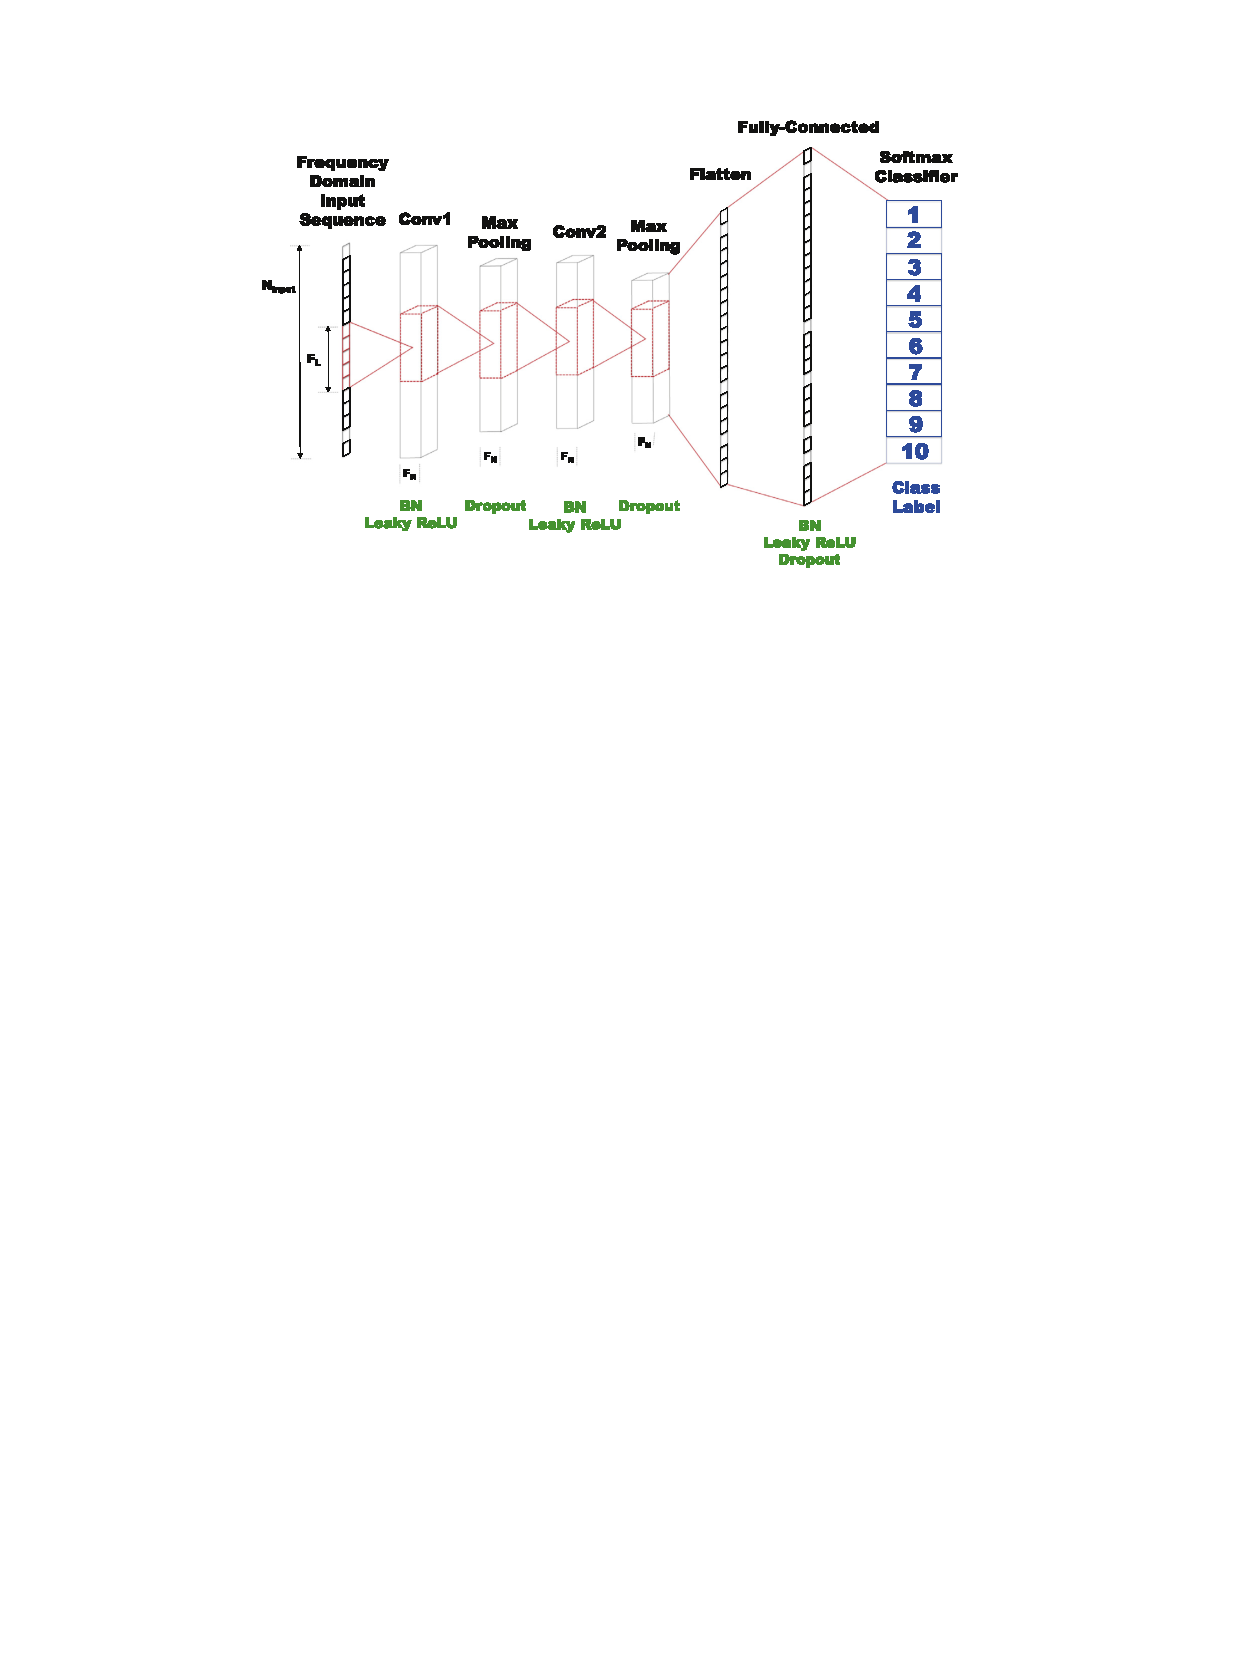
\includegraphics[width=.75\textwidth]{models_state_of_the_art/Deep_distance_metric_learning_model.pdf}
  \caption{Deep distance metric learning model \cite{Li2018}}
  \label{fig:Deep_distance_metric_learning_model}
\end{figure}

Li et al suggest to optimize the model such that the distance between samples of the same class is minimized and maximized between those of different classes. This increases the separability between as well as the compactness within the classes, which makes the algorithm more robust against environmental noises. In order to calculate the intra- and inter-class distances the expectation and variance of source domain samples belonging to the same class need so be measured in the feature maps of interest:

\begin{equation}
    \begin{aligned}
       &D_{inter} = |E[f^{(m)}x^{(i)}]-E[f^{(m)}x^{(j)}]|_{2}-\sqrt{Var[f^{(m)}x^{(i)}]}-\sqrt{Var[f^{(m)}x^{(j)}]}\\
       &D_{intra} = 
        \sum_{i=1}^{N_{class}} \sqrt{Var[x^{(i)}]},
    \end{aligned}
\end{equation}

where $x^{(k)}$ denotes the raw input sample of class k, $N_{class}$ is the number of classes, $f^{(m)}x^{(k)}$ denotes the feature representation of the input sample $x^{(k)}$ in the m-th layer and $E[f^{(m)}x^{(i)}]$ and $Var[x^{(i)}]$ are the  expectation and variance of this feature map. Optimizing the network with $J_{Cluster} = - D_{inter} + \eta D_{intra}$ reduces the inter- and maximizes the intra-class distance. Since $J_{Cluster}$  requires labels for each sample the optimization is restricted to source domain data. Furthermore, Li et al applies a MMD loss to reduce the discrepancy between target and source domain: 

\begin{equation}
    \begin{aligned}
    J_{MMD,m} = MMD_{k}(P^{f(m)}, Q^{f(m)}),
    \end{aligned}
\end{equation}

where $P^{f(m)}$ and $Q^{f(m)}$ denote the representation of source and target samples in the m-th hidden layer. Lastly, a cross entropy loss in the final layer optimizes the network to classify the source samples correctly. In total the network is optimized with the following weighted average of losses: 

\begin{equation}
    \begin{aligned}
    J_{total} = \alpha J_{Cluster} + \beta J_{MMD} + \gamma J_{CE}, 
    \end{aligned}
\end{equation}
where $J_{Cluster}$ is the cluster loss, $J_{MMD}$ the MMD loss,  $J_{CE}$ the cross entropy loss and $\alpha$, $\beta$ and $\gamma$ are the weights for calculating the weighted average \cite{Li2018}.


\subsection{Deep convolutional transfer learning network (DCTLN)}
Predictive maintenance of rolling bearing is a task with high demand in the industry. Guo et al \cite{Guo2019} propose a health condition classifier which reduces the domain discrepancy by applying a MMD loss and using a domain classifier. The architecture of the model is visualized in fig. \ref{fig:DCTLN_model}. Features are extracted by a CNN containing 16 layers including one input layer, six convolutional layers, six pooling layers, two fully connected layers, and one output layer. Each convolutional layer is combined with a consecutive pooling layer.


The model is optimized with a combination of three losses
\begin{itemize}
    \item [1.] Reduce the health condition classification loss on the source domain data
    \item [2.] Maximize the Domain classification loss on the source and target domain 
    \item [3.] Minimize the MMD distance between the source and target domain in the FC2 layer
\end{itemize}

\textbf{Objective 1}: By applying the cross entropy loss the model training minimizes the health condition classification error on the source domain data.

\textbf{Objective 2}: The domain classifier processes the features in the layer FC3 and tries to predict the corresponding domain of each sample. The model is trained to extract domain independent features such that the error of the domain classifier is increased.

\textbf{Objective 3}: The MMD loss is applied in the feature map FC2. The model is optimized to decrease the domain discrepancy and to extract more domain invariant features in FC2 \cite{Guo2019}. 

\begin{figure}[H]
  \centering
  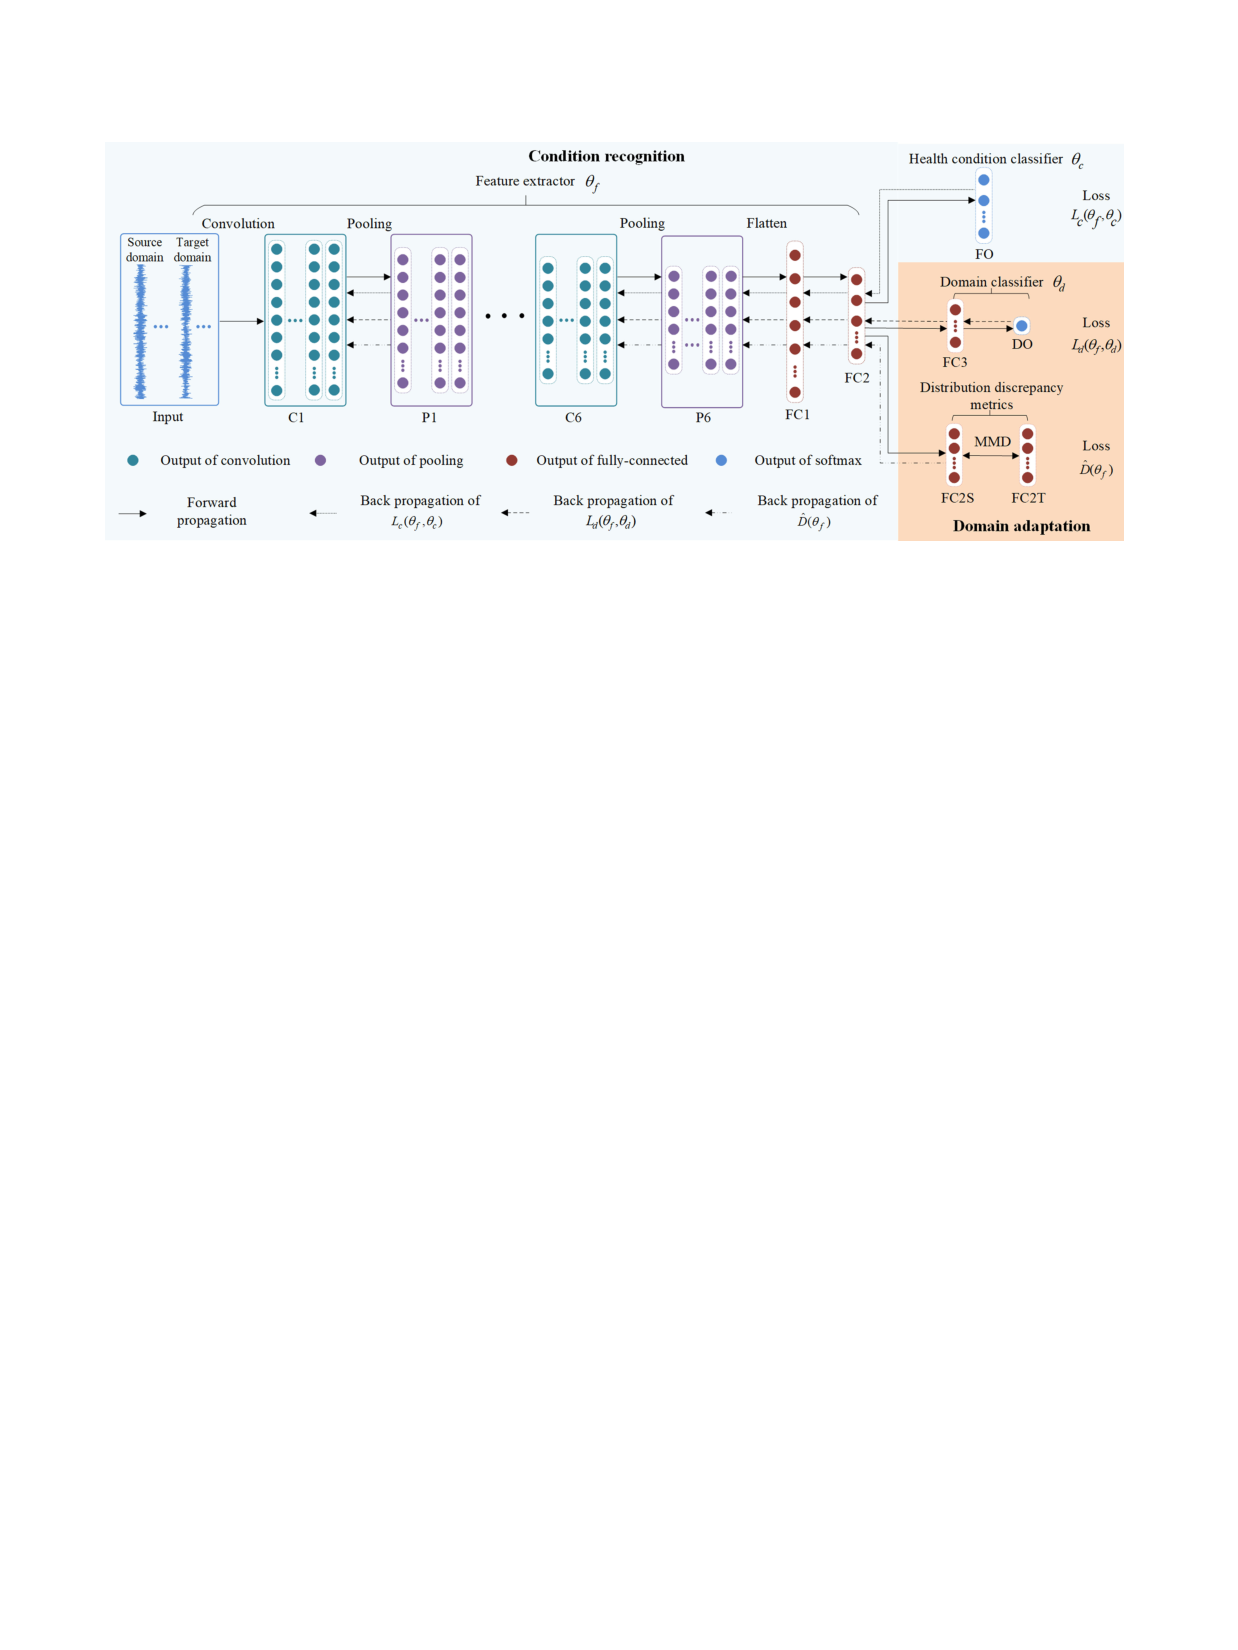
\includegraphics[width=1\textwidth]{models_state_of_the_art/DCTLN_model.pdf}
  \caption{DCTLN model \cite{Guo2019}}
  \label{fig:DCTLN_model}
\end{figure}

\subsection{Domain Conditioned Adaptation Network (DCAN)}
Most domain adaption approaches reduce the domain discrepancy in task-specific layers but use a shared feature extractor backbone across all domains. Li et al \cite{li2020} assume that, if the domain discrepancy is tremendously large, these methods can only reduce the domain discrepancy, but not fundamentally eliminate it. Since the source and target domains are distributed differently and a supervised training is just possible with the source domain data, the CNN learns to extract features which are sensitive for the source domain but might not work well classifying target domain data. Li et al recommend to extract domain-specific and -independent features in the feature extractor backbone. Since the source and target domains are correlated to some extend, it makes sense to extract domain-independent features to profit from the powerful feature extraction learned from the source when processing target domain data. Additionally the model uses a feature extractor capturing domain-specific features in the convolutional layers to improve the cross-domain feature alignment in the task-specific layers. In a second stage, the extracted features are adjusted by the Domain Conditioned Feature Correction Module with the goal to reduce the domain discrepancy. Lastly, the model is optimized with a conventional supervised source and a newly proposed unsupervised target cross-entropy loss defined as following:

\begin{equation}
    \min_{G} L_{s} = -\frac{1}{n_{t}} \sum_{j=1}^{n_{t}} \sum_{k=1}^{C_{t}} G^{(k)}(\pmb{x}_{tj})logG^{(k)}(\pmb{x}_{tj}),
\end{equation}
where $G(\cdot)$ is the learned predictive model, $n_{t}$ is the number of source domain samples, $C_{n}$ are the classes present in source and target domain and $\pmb{x}_{t}$ are target samples.

The presented model is developed for computer vision applications and not predictive maintenance. Since predictive maintenance suffers from similar problems, this approach might be still be relevant. The model is visualized in fig. \ref{fig:DCAN_model}. In the following the two domain adaption modules are described in more detail \cite{li2020}. 

\subsubsection{Domain Conditioned Channel Attention Mechanism}
Li et al \cite{li2020} use ResNet as backbone network which allows easy implementation of domain conditioned channel attention module in it's residual block. In the latent feature maps the processed images are represented as $\pmb{X}_{t} = [X^{1}_{t},...,X^{C}_{t}] \in \mathbb{R}^{HxWxC}$,where H and W are the spatial dimension and C the number of image channels. First, a channel-wise global average pooling layer is applied which reduces the images to  $\pmb{g}_{t} = [g^{1}_{t},...,g^{C}_{t}] \in \mathbb{R}^{1x1xC}$. Afterwards, the data is split depending on its domain and passed through different fully connected layers. The upper flow is used for target and the lower flow for source domain samples. The two different source and target domain routes share parameters. For both domains the attention mechanism is learned jointly in order to learn activating different channels for the domains, which allows extracting enriched domain specific features. In the fully connected layers the dimension is first reduced with a ratio ${1x1x\frac{C}{r}}$ and later reconstructed to its original size ${1x1xC$. In this context Relu and Sigmoid functions are applied. The domain-wise feature selection is achieved by weighting the channels of the original feature $\pmb{X}_{s}$ and $\pmb{X}_{t}$ with the resulting channel attention vectors $\pmb{v}_{s}$ and $\pmb{v}_{t}$ from the Domain Conditioned Channel Attention Module:

\begin{equation}
    \begin{aligned}
        &\pmb{\tilde{X}}_{s} = \pmb{v}_{s} \odot \pmb{X}_{s} = [v_{s}^{1} \cdot X_{s}^{1}, ..., v_{s}^{C} \cdot X_{s}^{C}]\\
        &\pmb{\tilde{X}}_{t} = \pmb{v}_{t} \odot \pmb{X}_{t} = = [v_{t}^{1} \cdot X_{t}^{1}, ..., v_{t}^{C} \cdot X_{t}^{C}].
    \end{aligned}
\end{equation}

The convolutional layers are activated by the channel attention vectors allowing the model to independently learn the importance of each channel for the source and target domain \cite{li2020}.

\subsubsection{Domain Conditioned Feature Correction}
A feature correction block is placed after each of the L task-specific layers. At the feature correction blocks the data simultaneously passes through the regular network and the feature correction block, which consist of FC and Relu blocks. The feature correction block estimates the domain discrepancy in the feature representation of the corresponding task-specific layer:
\begin{equation}
    \Delta H_{l}(x_{t}) = H_{l}(x_{s}) - H_{l}(x_{t}),
\end{equation}
where $H_{l}(x_{s})$ and $H_{l}(x_{t})$ are the feature representations of the source and target domain samples in the task-specific layer L and $\pmb{x}_{s}$ and $\pmb{x}_{t}$ are source and target domain samples. The feature representation of this layer is then modified as following:
\begin{equation}
    \hat{H}_{l}(x_{t}) = H_{l}(x_{t}) + \Delta H_{l}(x_{t}).
\end{equation}
An MMD loss is applied in several latent feature maps described by $\hat{H}_{l}(x_{t})$ and $H_{l}(x_{s})$:

\begin{equation}
    L_{M}^{l} = |\frac{1}{n_s} \sum_{i=1}^{n_{s}} \phi(H_{l}(x_{si}) - \frac{1}{n_t} \sum_{i=1}^{n_{t}} \phi(\hat{H}_{l}(x_{ti}))|_{H_{\kappa}}^{2}, 
\end{equation}
where $H_{\kappa}$ is the reproducing kernel Hilbert space (RKHS) using the characteristic kernel $\kappa$ and corresponding feature map  $\phi$. The number of source and target samples is defined by $n_{s}$ and $n_{t}$. Reducing the domain discrepancy improves the feature transferability but also transfers noise and unimportant information between the domains, which destroys the structure of the source and target domain data, making the classification task more difficult. To avoid this over-transfer between source and target, the model should be enforced to keep the source data constant when passing through the feature correction blocks. Since $\Delta H_{l}(x_{s}) \approx 0$ would prevent the cross-domain feature correction a regularization term should tackle that problem:
\begin{equation}
    L_{reg}^{l} = \sum_{k=1}^{C_{n}}|\frac{1}{n_{s}^{k}} \sum_{x_{si} \in S^{k}} \phi(H_{l}(x_{si})) - \frac{1}{|R|} \sum_{x_{sj} \in R} \phi(\hat{H}_{l}(x_{sj}))|_{Hk}^{2}, 
\end{equation}
where $R$ is a random subset in the source domain samples and $S^{k}$ is the set of source domain samples belonging to class k \cite{li2020}.

\begin{figure}[H]
  \centering
  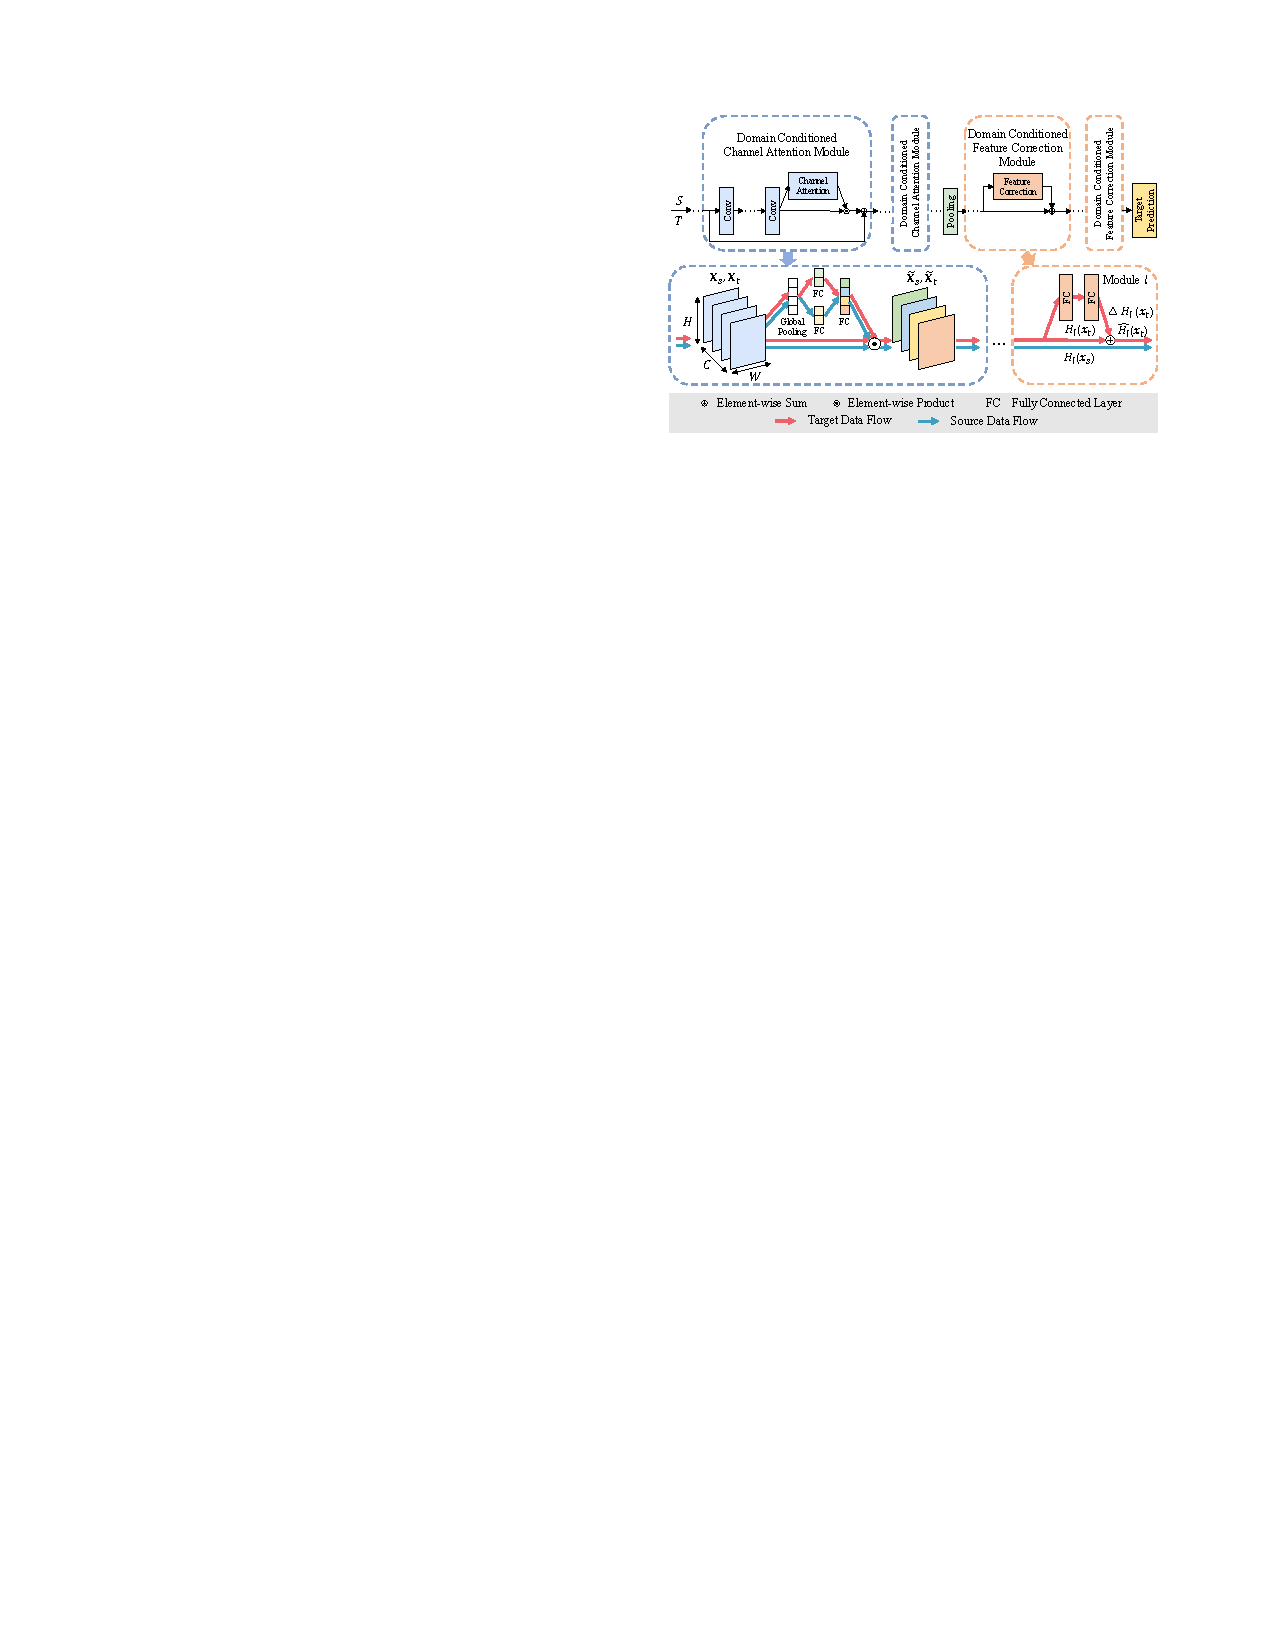
\includegraphics[width=1\textwidth]{models_state_of_the_art/DCAN_model.pdf}
  \caption{DCAN model \cite{li2020}}
  \label{fig:DCAN_model}
\end{figure}

\subsection{Deep belief networks}
A domain adaption algorithm based on DBNs which uses wavelet packet transforms (WTPs) as a pre-processing step was proposed by Zang et al \cite{Zhang2017}. Degradation of ball screws lead to decreasing stiffness in the system which increases vibrations. These characteristic vibration signals are therefore promising for evaluating the degradation state of the ball screws \cite{Zhang2017}. Zang et al apply WTPs, which are an expansion of the discrete wavelet transform, as a pre-processing step. This feature extraction technique considers variations in the temporal and frequency band energy \cite{Besbes2016}. The packet energy of the WPT shows an exponential increase trend with increasing degradation and is therefore a good indicator for the degradation level. In order to have a better basis for decisions, multi-sensor data fusion methods are used to synthesize data from different sources. The proposed method presented by Zang et al is visualized in fig. \ref{fig:Deep_belief_networks_model} and described the following step by step:

\begin{itemize}
    \item [1.] Collect N signals with sensors mounted at different machine positions.
    \item [2.] Calculate the frequency spectrum $\{f_{(1)}^{i}, ..., f_{(N)}^{i}\}_{i=1}^{M}$ for each of the N extracted time-domain signals using wavelet packet transforms, where M is the number of degradation samples.
    \item [3.] Fuse the frequency spectrum of the N signals $\{F^{i}\}_{i=1}^{M}$, with $F^{i}=f_{(1)}^{i} \cap ... \cap f_{(N)}^{i}$. The fused frequency spectrum is normalized by its dimension, which is expressed as $dim(F^{i})=\sum_{j=1,...,N} dim(f_{(j)}^{i})$.
    \item [4.] Pre-train the DBN by applying the regular RBM training (iteratively apply positive and negative phases) to each layer. The fused frequency spectra are used for the unsupervised training. 
    \item [5.] Separate the level of degradation in classes and obtain the output dimension of the model.
    \item [6.]  Fine-tune the deep belief network with the supervised back-propagation training algorithm. The error between the true and predicted degradation class should be minimized.
    \item [7.] Apply the model as intelligent degradation monitoring system to estimate the degradation level of unseen data samples \cite{Zhang2017}.
\end{itemize}

\begin{figure}[H]
  \centering
  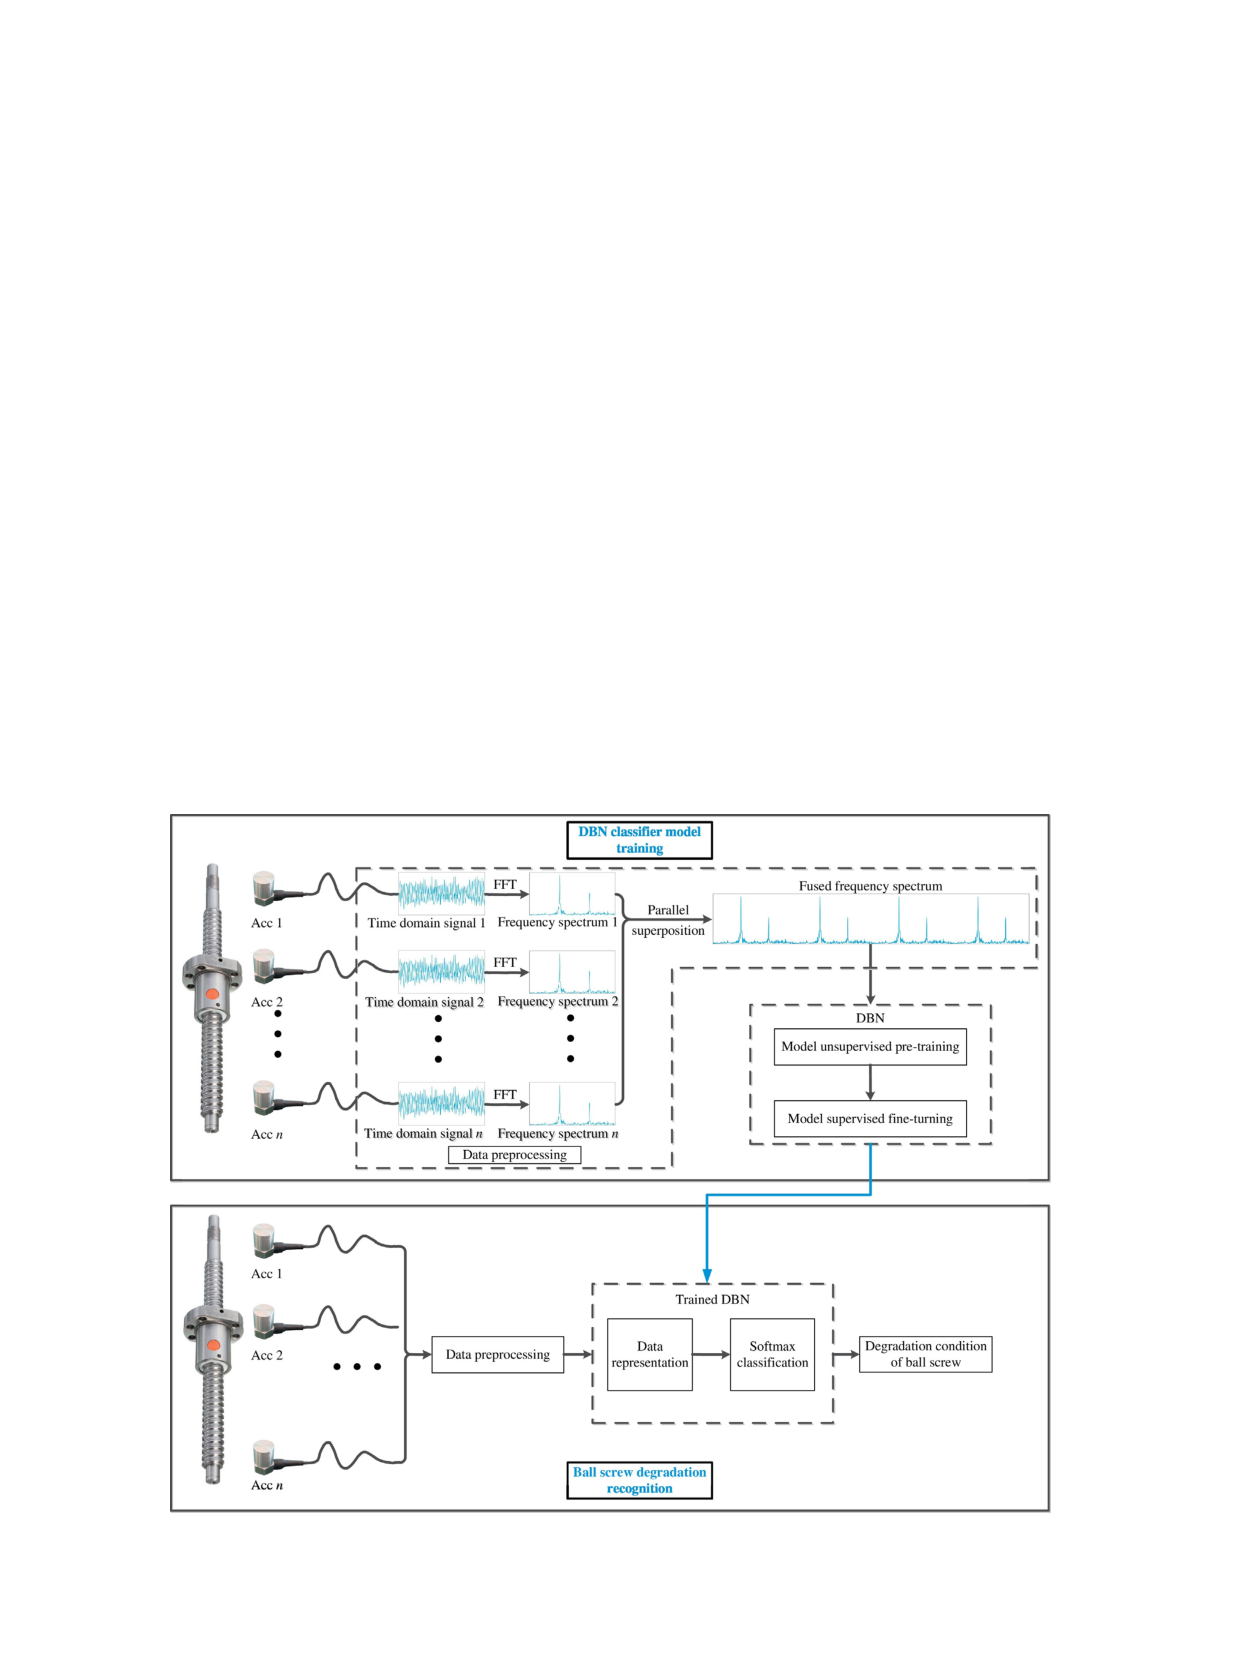
\includegraphics[width=1\textwidth]{models_state_of_the_art/Deep_belief_networks_model.pdf}
  \caption{Deep belief networks model \cite{Zhang2017}}
  \label{fig:Deep_belief_networks_model}
\end{figure}


\subsection{Wasserstein distance guided multi-adversarial networks (WDMAN)}
 Zhang et al \cite{Zhang2019} present a model for addressing the rolling bearing fault diagnosis under different working conditions. An adversial learning strategy enables the extraction of domain-independent features. The Wasserstein-distance is used to estimate the domain discrepancy. In general the proposed architecture consists of a CNN feature mapper and a subsequent classifier containing several fully connected layers. By applying the Wasserstein distance the domain discrepancy in the different fully connected layers is estimated with several domain critics. The whole model and the applied loss can be seen in fig. \ref{fig:WDMAN_model}. In a first step the feature mapper and classifier are optimized using a regular source cross entropy loss. In a second step the domain discrepancy is reduced by applying a transfer procedure of adversarial learning. In this phase the domain critics are updated by maximizing the feature mapper and minimizing the Wasserstein distance: 
 
 \begin{equation}
     L_{wd}(x^{s}, x^{t}) = \frac{1}{n^{s}} \sum_{x^{s} \in X^{s}} D(F(x^{s})) - \frac{1}{n^{t}} \sum_{x^{t} \in X^{t}} D(F(x^{t})),
 \end{equation}
 where $x^{s}$ and $x^{t}$ are the data samples drawn from the source domain $X^{s}$ and target domain $X^{t}$. In the fully connected layers $F(\cdot)$ is the transformation of the input samples to it's feature representation. Generally, the goal of the discriminators is to identify the domain of each sample and the feature mapper tries to extract features which are domain independent, which precludes the discriminator to predict the correct domain. To satisfy the Lipschitz constraint condition of Wasserstein distance an additional gradient penalty is applied: 

 \begin{equation}
     L_{gp}(\tilde{x}) = (|\nabla_{\tilde{x} \in P_{\tilde{x}}} D(\tilde{x})|_{2}-1)^{2}, 
 \end{equation}
 where $P_{\tilde{x}}$ is a distribution of samples coming from the line connecting a pair of points sampled from the source and target domain. In the adversarial learning the feature mapper and discriminators are optimized in an alternating procedure. Firstly, the domain critics are optimized to minimize the Wasserstein distance, which the feature mapper tries to maximize afterwards. The Wasserstein distance is extended with the gradient penalty. The adversial training can be described as following: 
 \begin{equation}
    \min_{\theta_{f}} \max_{\theta_{d}} (L_{wd} - \lambda L_{gp}), 
 \end{equation}
 where $\theta_{f}$ and $\theta_{d}$ are the parameters of the feature mapper and domain critics, and $\lambda$ is the penalty coefficient. The workflow of the model is described more detailed in fig. \ref{fig:WDMAN_workflow}
 \begin{figure}[H]
  \centering
  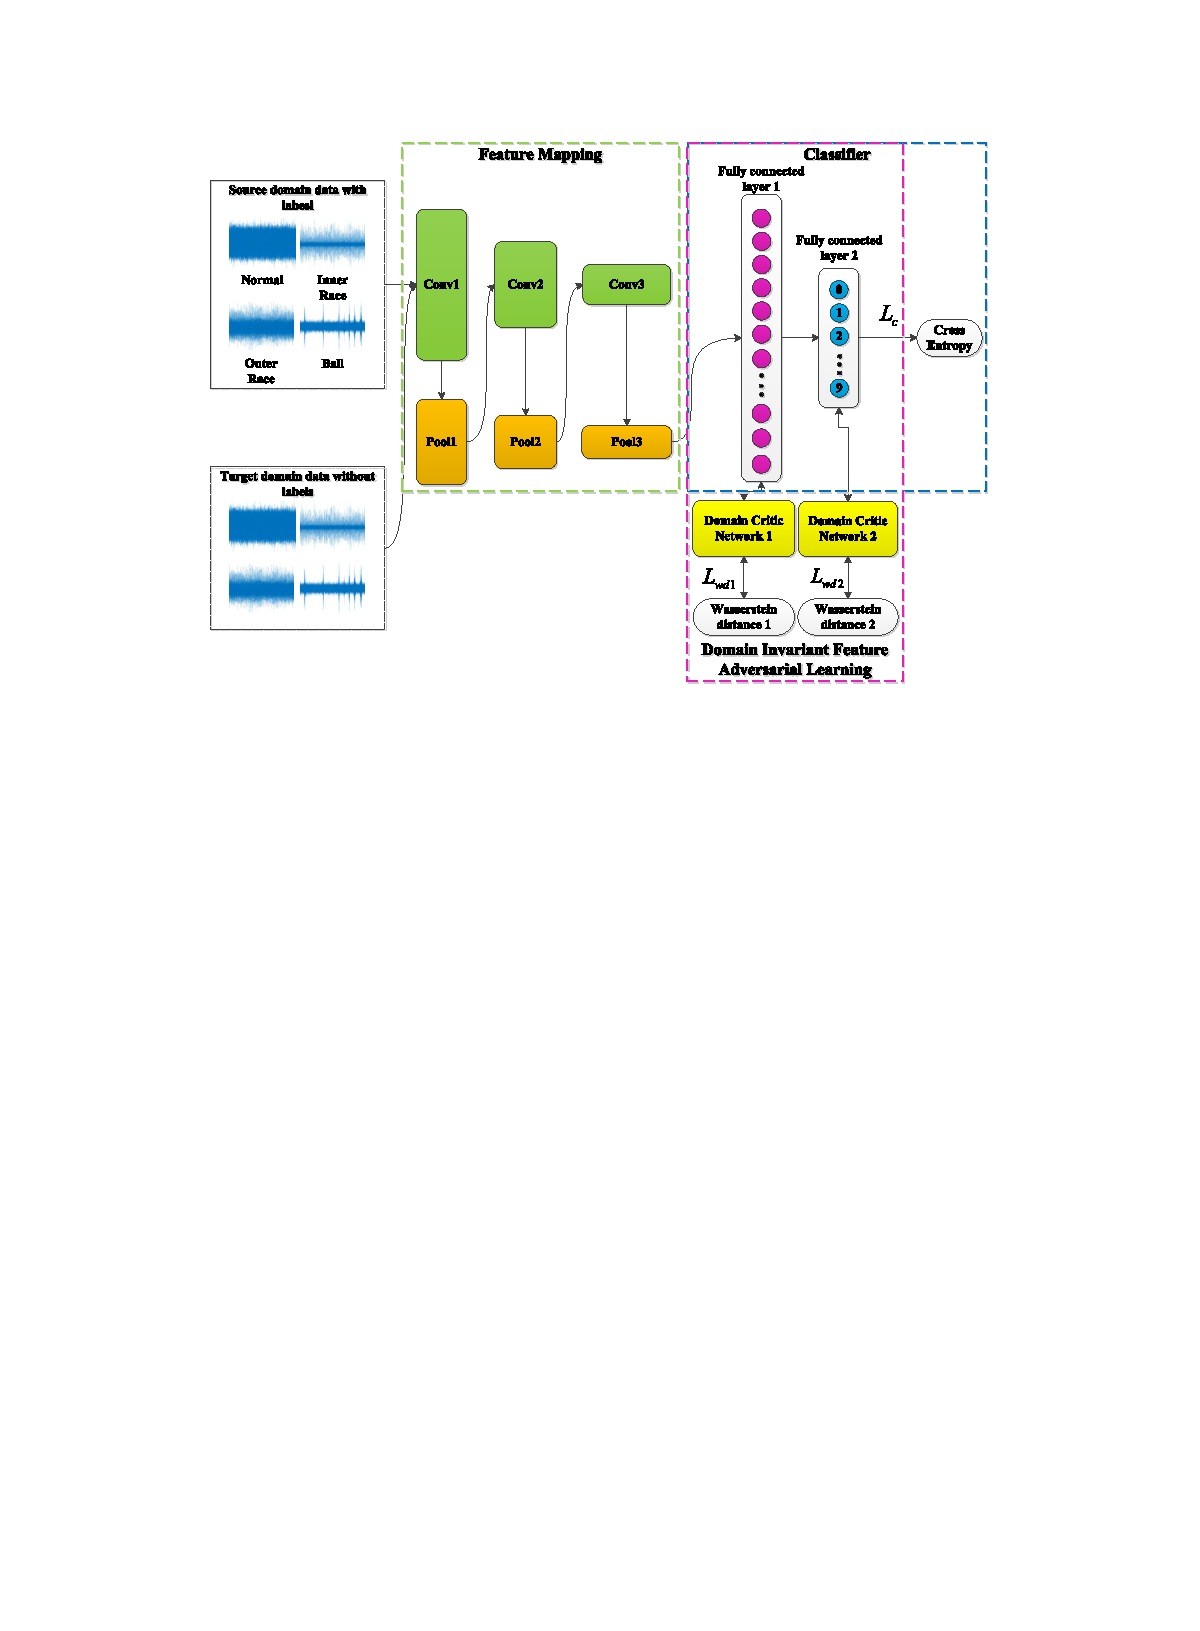
\includegraphics[width=1\textwidth]{models_state_of_the_art/WDMAN_model.pdf}
  \caption{WDMAN model \cite{Zhang2019}}
  \label{fig:WDMAN_model}
\end{figure}
 
  \begin{figure}[H]
  \centering
  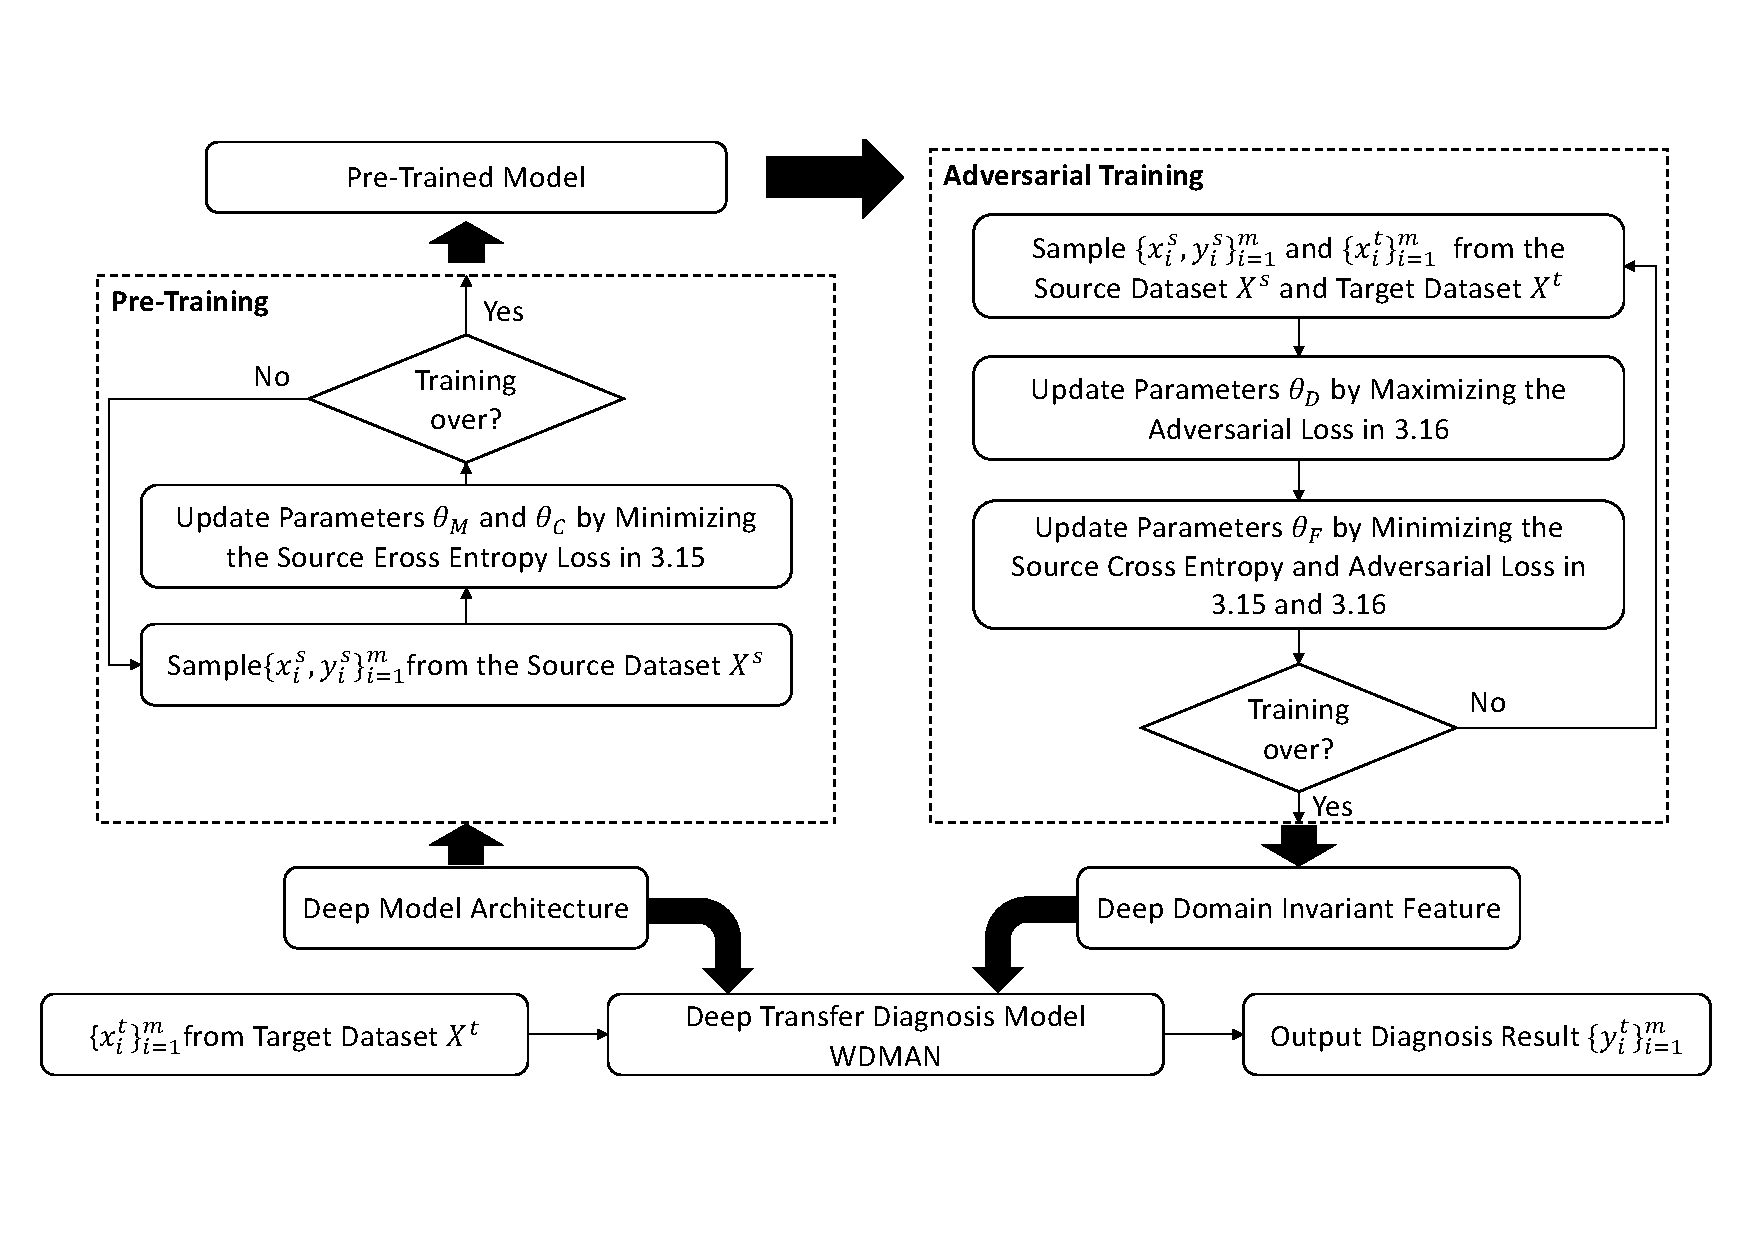
\includegraphics[width=.7\textwidth]{models_state_of_the_art/WDMAN_workflow.pdf}
  \caption{WDMAN workflow \cite{Zhang2019}}
  \label{fig:WDMAN_workflow}
\end{figure}
 
 
 
 
 
 
 
 
 
 
 
 